%!TEX root=../documentation-bachlorthesis-speicherarchitektur-lstucker.tex

\cleardoublepage
\chapter{Soll-Analyse}
Ziel ist es mit der Sollanalyse, den soll Zustandstand der Speicherinfrastruktur, welche die verschiedenen Szenerien der Datenwachstum und Datenzugriffe in den nächsten drei Jahren erfüllen soll zu beschreiben. 

Der Auftraggeber Selbst geht von einen Starken Wachstum im Bereichen der Datenmengen und Datenzugriffe aus welche das Szenario 3 am ehesten wieder spiegelt.

\section{Defintion}
\subsection{Evaluations Bewertungs Verfahren}
Für die das Evaluation bzw. Bewertung Verfahren wird das Analytische Hierachie-Prozess (AHP) Verfahren angewendet. AHP wurde in den siebziger Jahren von Thomas L. Saaty zur Lösung mehrkriterieller Entscheidungsprobleme entwickelt.

Der Entscheidungsprozesse ist beim AHP Analytisch und Hirachisch. Die Analyse beruht auf mathematischen und logischen Entschlüsse. Die Hirachie wird durch

Beim AHP werden die Priorität bzw. die Gewichtung jedes Element im vergleich zu den anderen Elemente mittels Evaluationsmatrix abgeleitet. In der Evaluationsmatrix werden die Elemente untereinander in Paarvergleich zu einander Bewertet. Für die Bewertung wird dazu die 9-Punkte-Bewertungsskale aus der \reftab{tab:9PBewertungsskala} bzw. der Umkehr Relation aus der \reftab{tab:UmgekehrteBewertungsskala} verwendet.

\begin{table}[htbp]
\caption{9-Punkte-Bewertungsskala}
\begin{tabular}{|c|L{3.5cm}|L{8.5cm}|}
\hline
\multicolumn{1}{|l|}{} & Definition & Interpretation \\ \hline
 1 &  gleiche Bedeutung &  Beide verglichenen Elemente haben die gleiche ""Bedeutung für das nächsthöhere Element. \\ \hline
3 &  etwas grossere "" ""Bedeutung & 
Erfahrung und Einschätzung sprechen für eine ""
etwas größere Bedeutung eines Elements im 
Vergleich zu einem anderen \\ \hline
5 &  erheblich grössere "" Bedeutung & 
Erfahrung und Einschätzung sprechen für eine "" 
erheblich größere Bedeutung eines Elements im ""
Vergleich zu einem andere \\ \hline
7 &  sehr viel grössere ""Bedeutung & 
Die sehr viel größere Bedeutung eines Elements 
hat sich in der Vergangenheit klar gezeigt. \\ \hline
9 &  absolut dominierend &  Es handelt sich um den größtmöglichen ""
Bedeutungsunterschied zwischen zwei 
Elemente \\ \hline
\multicolumn{1}{|l|}{2,4,6,8} & Zwischenwerte &  \\ \hline
\end{tabular}
\label{tab:9PBewertungsskala}
\end{table}

\begin{table}[htbp]
\caption{Umgekehrte Relationen der Bewertungsskala}
\begin{tabular}{|c|L{3.5cm}|L{7.3cm}|}
\hline
\multicolumn{1}{|l|}{} & Definition & Intepretation \\ \hline
1 & gleiche Bedeutung & Beide verglichenen Elemente haben die gleiche 
Bedeutung für das nächsthöhere Element. \\ \hline
 1/3 & etwas geringere Bedeutung & Erfahrung und Einschätzung sprechen für eine 
etwas geringere Bedeutung eines Elements im 
Vergleich zu einem anderen.  \\ \hline
 1/5 & erheblich geringere Bedeutung & 
Erfahrung und Einschätzung sprechen für eine 
erheblich geringere Bedeutung eines Elements im 
Vergleich zu einem anderen \\ \hline
 1/7 & sehr viel geringere Bedeutung & 
Die sehr viel geringere Bedeutung eines Elements 
hat sich in der Vergangenheit klar gezeigt \\ \hline
 1/9 & absolut unterlegen & Es handelt sich um den größtmöglichen 
Bedeutungsunterschied zwischen zwei 
Elementen \\ \hline
\multicolumn{1}{|l|}{1/2, 1/4, 1/6, 1/8} & Zwischenwerte &  \\ \hline
\end{tabular}
\label{tab:UmgekehrteBewertungsskala}
\end{table}

In dieser Arbeit wurde für die Berechnung der Priorität die Methode für die Vereinfachte Berechnung eingesetzt, wie diese in der \reftab{tab:Gewichtsberechnung} dargestellt ist.
Beim der Vereinfachte Berechnung werde die Paarvergleichswerte auf eine vergleichbare Basis gebracht. Dazu werden die Spaltensummen ($c_i$) der Evaluationsmatrix bestimmt. Dann werden diese auf 1 normiert, indem man jeden Paarvergleichswert durch die Spaltensumme dividiert. Anschließend werden aus 
der normalisierten Matrix die Zeilensummen ($r_i$) gebildet und durch die Anzahl für das jeweilige Element 
ergibt. 

\begin{table}[htbp]
\caption{Gewichtsberechnung mit der Eigenvektormethode }
\begin{tabular}{l|llll|llll|l|l}
 & \multicolumn{ 4}{c|}{Evaluationsmatrix} & \multicolumn{ 4}{c|}{Normalisierung} &  & Gewicht \\ 
 & $a_1$ & $a_2$ & \dots & $a_n$ & $a_1$ & $a_2$ & \dots & $a_n$ & $r_i$ &  $w$ \\ \hline
$a_1$ & $a_1_1=1$ & $a_1_2$ & \dots & $a_1_n$ & $\frac{a_1_1}{c_1}$  & $\frac{a_1_2}{c_1}$  &  \dots & $\frac{a_1_n}{c_n}$  & $r_1$  & $w_1=\frax{r_1}{n}$  \\ 
$a_2$ & $a_2_1 = \frac{1}{a_1_2}$ & 1 &  \dots & $a_2_n$  &  $\frac{a_2_1}{c_1} & $\frac{a_2_2}{c_2}$  & \dots &  $\frac{a_2_n}{c_n}$ &  $r_2$ & $w_2 = \frac{r_2}{n}$  \\ 
\vdots & \vdots & \vdots  &  &  \vdots&\vdots  & \vdots &  & \vdots & \vdots &\vdots  \\ 
$a_n$ & $a_n_1 =\frac{1}{a_1_n}$ & $a_2_n$ & \dots  & $a_n_n = 1$  & $\frac{a_n_1}{c_1}$  & $\frac{a_n_2}{c_s}$ & \dots  & $\frac{a_n_n}{c_n}$  & $r_n$ & $w_n = \frac{r_n}{n}$ \\ \hline
$c_i$ & $c_1 = \displaystyle\sum\limits_{i=1}^n a_i_1$ & $c_2 = \displaystyle\sum\limits_{i=1}^n a_i_2$ & \dots & $c_n$ & 1 & 1 & \dots & 1 & $n$ & 1 \\ 
\end{tabular}
\label{tab:Gewichtsberechnung}
\end{table}

\subsection{Auswahl der Kriterien}

\begin{center}
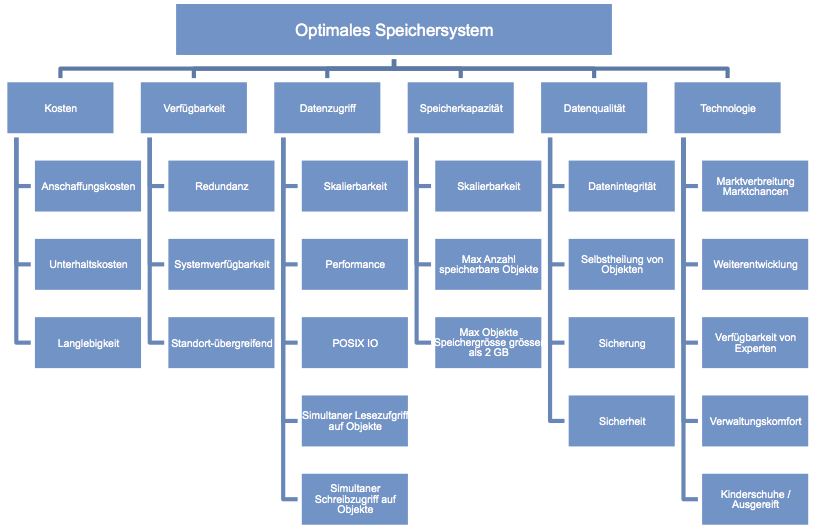
\includegraphics[width=\linewidth, keepaspectratio = true]{media/ahp_kirterienbaum.png}
\mycaption{figure}{\label{abb:AHPKriterienbaum} Optimales Speichersystem Kriterien}
\end{center}

\section{Szenario 1 - Schwaches Datenvolumen und Datenzugriff Wachstum}
Dieses Szenario beschreibt den Sollzustand, wenn sich das Datenwachstum und Datenzugriffs Wachstum im gleichen Umfang wie in der Ist-Analyse weiter entwickelt. Was der Fall währe, wenn sich die Anzahl der Kunden auf den Bestehenden Niveau bleibt und der Bedarf an Speicherkapazität beziehungsweise die Aufträge zur Aufbereitung der Bilddaten gleich weiter entwickeln wie bisher.

Anzahl Kunden: 10 (Annahme)

Datenwachstum in Prozent pro Monat: 5\% 

Datenwachstum in Tebibyte pro Monat: 0.19 Tebibyte

Speichervolumen in 36 Monaten: 9.34 Tebibyte

\subsection{Verfügbarkeit}
Die Verfügbarkeit soll mindestens dem AEC-2 Standard von Harvard Research entsprechen. Dass bedeutet die Verfügbarkeit der Applikation beziehungsweise der Daten darf nur innerhalb festgelegter Zeit beziehungsweise zur Hauptbetriebszeit minimal unterbrochen werden.

Die Daten müssen mindesten in einfacher Redundanz vorhanden sein. 

Die Online-Daten müssen nicht standortübergreifend verfügbar sein.

\subsection{Datenzugriff}
Die bestehende Speicherarchitektur konnte die bisherigen Datenzugriffe mit einem Web-Server bisher zufriedenstellend erfüllen. Es wird davon ausgegangen, dass sich die Anzahl Datenzugriff für die Bildaufbereitung und Speicherung von neuen Bilddaten, nicht weiter steigert.

Der \gls{POSIX} zugriff soll nach Möglichkeit unterstützt werden.

Es muss keine simultaner Lesezugriff bzw. Schreibzugriff auf Objekte von Mehren Web-Server gewährleistet werden.

\subsection{Speicherkapazität}
Geht man von einem Datenwachstum von 5\% pro Monat aus, bzw. 0.19 Tebibyte, wird das Speichervolumen für das Speichern aller Bilddaten 9.34 Tebibyte betragen. Rechnet man mit einer zusätzlichen Reserve von 40\% für Eventuelles zusätzliches Wachstum oder Migration Reserve, muss das Speichersystem mindestens 13 Tebibyte exklusive der Datenredundanz an Speicherkapazität zur Verfügung stellen können.

Das Speichersystem soll 400'000 speicherbare Objekte unterstützen.

Das Speichersystem muss die Speicherung von Objekten von mindestens 2 Gibibyte grösse unterstützen.

\subsection{Datenqualität}

Die Selbstheilung von Objekten muss nicht unterstützen werden und gilt als optional.

Die Sicherung und Wiederherstellung der Daten aus einer Sicherung muss möglich sein. Die Sicherung der Daten muss bei Fehlenden standortübergreifende Verfügbarkeit der Daten an einen anderen Standort möglich sein.

Die Sicherheit der Daten wird über d

%\subsection{Daten Integrität}
%Dem Kunden wird einen Qualität Standard gewährleistet, die Original gespeicherten Daten, sollen vor Veränderung geschützt werden, aus diesen Grund soll die Daten Integrität beim Zugriff auf die Original Daten sichergestellt sein.


\subsection{AHP Gewichtung}
\begin{table}[htbp]
\caption{Top Kriterien Szenario 1}
\begin{tabular}{|l|c|c|c|c|c|r|r|}
\hline
\multicolumn{ 1}{|c|}{} & \multicolumn{ 5}{c|}{Evalutations Matrix} & \multicolumn{1}{l|}{} & \multicolumn{1}{l|}{Gewicht} \\ \cline{ 2- 8}
\multicolumn{ 1}{|c|}{} & K & V & P & S & D & \multicolumn{1}{c|}{r} & \multicolumn{1}{c|}{w} \\ \hline
Kosten (K) & \textbf{1} & 2 & 3 & 1 & 1 & 1.131 & 0.226 \\ \hline
Verfügbarkeit (V) &  1/2 & \textbf{1} & 5 &  1/3 &  1/8 & 0.569 & 0.114 \\ \hline
Performance (P) &  1/3 &  1/5 & \textbf{1} &  1/4 &  1/7 & 0.257 & 0.051 \\ \hline
Speicherkapazität (S) & 1 & 3 & 4 & \textbf{1} &  1/2 & 1.071 & 0.214 \\ \hline
Datenqualität (D) & 1 & 8 & 7 & 2 & \textbf{1} & 1.972 & 0.394 \\ \hline  \hline
Ci & \multicolumn{1}{r|}{3.833} & \multicolumn{1}{r|}{14.200} & \multicolumn{1}{r|}{20.000} & \multicolumn{1}{r|}{4.583} & \multicolumn{1}{r|}{2.768} & 5 & 1 \\ \hline 
\end{tabular}
\label{AHPTopKriterienS1}
\end{table}


\begin{table}[htbp]
\caption{Kosten Szenario 1}
\begin{tabular}{|l|c|c|c|r|r|}
\hline
\multicolumn{ 1}{|c|}{Wirtschaftlichkeit} & \multicolumn{ 3}{c|}{Evalutations Matrix} & \multicolumn{1}{l|}{} & \multicolumn{1}{l|}{Gewicht} \\ \cline{ 2- 6}
\multicolumn{ 1}{|c|}{} & A & U & L & \multicolumn{1}{c|}{r} & \multicolumn{1}{c|}{w} \\ \hline
Anschaffung (A) & \textbf{1} &  1/4 &  1/3 & 0.368 & 0.123 \\ \hline
Unterhaltskosten (U)  & 4 & \textbf{1} & 2 & 1.671 & 0.557 \\ \hline
Langlebigkeit (L) & 3 &  1/2 & \textbf{1} & 0.961 & 0.320 \\ \hline \hline 
Ci & \multicolumn{1}{r|}{8.00} & \multicolumn{1}{r|}{1.750} & \multicolumn{1}{r|}{3.333} & 3 & 1 \\ \hline
\end{tabular}
\label{AHPKostenS1}
\end{table}

\begin{table}[htbp]
\caption{Verfügbarkeit Szenario 1}
\begin{tabular}{|p{7.1cm}|c|c|c|r|r|}
\hline
\multicolumn{ 1}{|c|}{Verfügbarkeit} & \multicolumn{ 3}{c|}{Evalutations Matrix} & \multicolumn{1}{l|}{} & \multicolumn{1}{l|}{Gewicht} \\ \cline{ 2- 6}
\multicolumn{ 1}{|c|}{} & R & SV & St & \multicolumn{1}{c|}{r} & \multicolumn{1}{c|}{w} \\ \hline
Redundanz (R) & \textbf{1    } & 8     & 3     & 1.971 & 0.657 \\ \hline
Systemverfügbarkeit (SV) &  1/8 & \textbf{1} &  1/5 & 0.205 & 0.068 \\ \hline
Standortübergreifend (St) &  1/3 & 5     & \textbf{1} & 0.824 & 0.275 \\ \hline \hline
Ci & \multicolumn{1}{r|}{1.458} & \multicolumn{1}{r|}{14.00} & \multicolumn{1}{r|}{4.200} & 3 & 1 \\ \hline
\end{tabular}
\label{AHPVerfügbarkeitS1}
\end{table}


\begin{table}[htbp]
\caption{Datenzugriff Szenario 1}
\begin{tabular}{|p{4.5cm}|c|c|c|c|c|r|r|}
\hline
\multicolumn{ 1}{|c|}{Datenzugriff} & \multicolumn{ 5}{c|}{Evalutations Matrix} & \multicolumn{1}{l|}{} & \multicolumn{1}{l|}{Gewicht} \\ \cline{ 2- 8}
\multicolumn{ 1}{|c|}{} & Sk & P & PIO  & L & S & \multicolumn{1}{c|}{r} & \multicolumn{1}{c|}{w} \\ \hline
Skalierbarkeit (Sk) & \textbf{1} & 2 & 8 & 4 & 5 & 2.193 & 0.439 \\ \hline
Performance (P) &  1/2 & \textbf{1} & 5 &  1/2 &  1/3 & 0.649 & 0.130 \\ \hline
POSIX IO (PIO) &  1/8 &  1/5 & \textbf{1} &  1/9 &  1/7 & 0.152 & 0.030 \\ \hline
Simultaner Lesezufgriff 
auf Objekte (L) &  1/4 & 2 & 9 & \textbf{1} & 3 & 1.149 & 0.230 \\ \hline
Simultaner Schreibzugriff
 auf Objekte (S) &  1/5 & 3 & 7 &  1/3 & \textbf{1} & 0.857 & 0.171 \\ \hline \hline
Ci & \multicolumn{1}{r|}{2.075} & \multicolumn{1}{r|}{8.200} & \multicolumn{1}{r|}{30.00} & \multicolumn{1}{r|}{5.944} & \multicolumn{1}{r|}{9.476} & 5 & 1 \\ \hline
\end{tabular}
\label{AHPDatenzugriffS1}
\end{table}

\begin{table}[htbp]
\caption{Speicherkapazität Szenario 1}
\begin{tabular}{|p{7.1cm}|c|c|c|r|r|}
\hline
\multicolumn{ 1}{|c|}{Speicherkapazität } & \multicolumn{ 3}{c|}{Evalutations Matrix} & \multicolumn{1}{l|}{} & \multicolumn{1}{l|}{Gewicht} \\ \cline{ 2- 6}
\multicolumn{ 1}{|c|}{} & S & A & G & \multicolumn{1}{c|}{r} & \multicolumn{1}{c|}{w} \\ \hline
Skalierbarkeit (S) & \textbf{1} & 1 & 9 & 1.498 & 0.499 \\ \hline
Max Anzahl speicherbare Objekte (A) & 1 & \textbf{1} & 6 & 1.310 & 0.437 \\ \hline
Max Objekt Speichergrösse grösser 2GB (G) &  1/9 &  1/6 & \textbf{1} & 0.192 & 0.064 \\ \hline \hline
Ci & \multicolumn{1}{r|}{2.111} & \multicolumn{1}{r|}{2.167} & \multicolumn{1}{r|}{16.00} & 3 & 1 \\ \hline
\end{tabular}
\label{AHPSpeicherkapazitätS1}
\end{table}


\begin{table}[htbp]
\caption{Datenqualität Szenario 1}
\begin{tabular}{|l|c|c|c|c|r|r|}
\hline
\multicolumn{ 1}{|c|}{Datenqualität} & \multicolumn{ 4}{c|}{Evalutations Matrix} & \multicolumn{1}{l|}{} & \multicolumn{1}{l|}{Gewicht} \\ \cline{ 2- 7}
\multicolumn{ 1}{|c|}{} & I & H & B & S & \multicolumn{1}{c|}{r} & \multicolumn{1}{c|}{w} \\ \hline
Datenintegrität (I) & \textbf{1} & 9 & 3 & 7 & 2.316 & 0.579 \\ \hline
Selbstheilung von Objekten (H) &  1/9 & \textbf{1} &  1/6 &  1/3 & 0.186 & 0.046 \\ \hline
Sicherung (B) &  1/3 & 6 & \textbf{1} & 5 & 1.130 & 0.282 \\ \hline
Sicherheit (S) &  1/7 & \multicolumn{1}{r|}{3    } &  1/5 & \textbf{1} & 0.369 & 0.092 \\ \hline  \hline
Ci & \multicolumn{1}{r|}{1.587} & \multicolumn{1}{r|}{19.00} & \multicolumn{1}{r|}{4.367} & \multicolumn{1}{r|}{13.333} & 4 & 1 \\ \hline
\end{tabular}
\label{AHPDatenqualitätS1}
\end{table}

\begin{table}[htbp]
\caption{Technologie Szenario 1}
\begin{tabular}{|p{3.9cm}|c|c|c|c|c|r|r|}
\hline
\multicolumn{ 1}{|c|}{Technologie} & \multicolumn{ 5}{c|}{Evalutations Matrix} & \multicolumn{1}{l|}{} & \multicolumn{1}{l|}{Gewicht} \\ \cline{ 2- 8}
\multicolumn{ 1}{|c|}{} & M & W & E & V & K & \multicolumn{1}{c|}{r} & \multicolumn{1}{c|}{w} \\ \hline
Marktverbreitung / Marktchancen (M) & \textbf{1} &  1/7 & 1 & 3 &  1/9 & 0.363 & 0.073 \\ \hline
Weiterentwicklung (W) & 7 & \textbf{1} & 5 & 4 &  1/9 & 1.067 & 0.213 \\ \hline
Verfügbarkeit von Experten (E) & 1 &  1/5 & \textbf{1} & 2 &  1/9 & 0.316 & 0.063 \\ \hline
Verwaltungskomfort (V) &  1/3 & \multicolumn{1}{r|}{ 1/4} &  1/2 & \textbf{1} &  1/9 & 0.202 & 0.040 \\ \hline
Kinderschuhe Ausgereift (K) & 9 & 9 & 9 & 9 & \textbf{1} & 3.052 & 0.610 \\ \hline  \hline
Ci & \multicolumn{1}{r|}{18.333} & \multicolumn{1}{r|}{10.593} & \multicolumn{1}{r|}{16.500} & \multicolumn{1}{r|}{19.00} & \multicolumn{1}{r|}{1.444} & 5 & 1 \\ \hline
\end{tabular}
\label{AHPTechnologieS1}
\end{table}



\section{Szenario 2 - Starkes Wachstum Daten / schwaches Wachstum der Abfragen}
Dieses Szenario beschreib den Soll-Zustand, wenn sich das Datenwachstum im Vergleich zum Ist-Zustand stark steigert, aber der Datenzugriff auf gleichem Niveau hält wie in der Ist-Analyse hält. Dieses Szenario würde eintreffen, wenn sich die Kunden Anzahl oder die Anzahl Bilddaten pro Kund stark steigert, jedoch die Anzahl Aufträge für die Aufbereitung der Daten für den Druck gleich bleiben würde.

Datenwachstum in Prozent pro Monat: 

Datenwachstum in Tebibyte pro Monat: 6 Tebibyte

Speichervolumen in 36 Monaten: 218,5 Tebibyte

Bilder mit einer Speichervolumen von 1 Gigibyte: 221'184

\subsection{Verfügbarkeit}
Die Verfügbarkeit soll mindestens dem AEC-2 Standard von Harvard Research entsprechen. Dass bedeutet die Verfügbarkeit der Applikation beziehungsweise der Daten darf nur innerhalb festgelegter Zeit beziehungsweise zur Hauptbetriebszeit minimal unterbrochen werden.

Die Daten müssen mindesten in einfacher Redundanz gespeichert sein. 

Die Online-Daten müssen nicht standortübergreifend verfügbar sein.

\subsection{Datenzugriff}
Die bestehende Speicherarchitektur konnte die bisherigen Datenzugriffe mit einem Web-Server bisher zufriedenstellend erfüllen. Es wird davon ausgegangen, dass sich die Anzahl Datenzugriff für die Bildaufbereitung und Speicherung von neuen Bilddaten, nicht weiter steigert.

Der \gls{POSIX} zugriff soll nach Möglichkeit unterstützt werden.

Es muss keine simultaner Lesezugriff bzw. Schreibzugriff auf Objekte von Mehren Web-Server gewährleistet werden.

\subsection{Speicherkapazität}
Geht man von einem Datenwachstum von 6 Tebibyte pro Monat aus, wird das Speichervolumen für das Speichern aller Bilddaten nach 36 Monaten 218,5 Tebibyte betragen. Rechnet man mit einer zusätzlichen Reserve von 40\% für Eventuelles zusätzliches Wachstum oder Migration Reserve, muss das Speichersystem mindestens 306 Tebibyte exklusive der Datenredundanz an Speicherkapazität zur Verfügung stellen können.

Das Speichersystem soll 9'500'000 speicherbare Objekte unterstützen.

Das Speichersystem muss die Speicherung von Objekten von mindestens 2 Gibibyte grösse unterstützen

\subsection{Datenqualität}
Die Selbstheilung von Objekten muss nicht unterstützen werden und gilt als optional.

Die Sicherung und Wiederherstellung der Daten aus einer Sicherung muss möglich sein. Die Sicherung der Daten muss bei Fehlenden standortübergreifende Verfügbarkeit der Daten an einen anderen Standort möglich sein.

%\subsection{Daten Integrität}
%Dem Kunden wird einen Qualität Standard gewährleistet, die Original gespeicherten Daten, sollen vor Veränderung geschützt werden, aus diesen Grund soll die Daten Integriät beim Zugriff auf die Original Daten sichergestellt sein.


\subsection{AHP Gewichtung}
\begin{table}[htbp]
\caption{Top Kriterien Szenario 2}
\begin{tabular}{|l|c|c|c|c|c|r|r|}
\hline
\multicolumn{ 1}{|c|}{} & \multicolumn{ 5}{c|}{Evalutations Matrix} & \multicolumn{1}{l|}{} & \multicolumn{1}{l|}{Gewicht} \\ \cline{ 2- 8}
\multicolumn{ 1}{|c|}{} & K & V & P & S & D & \multicolumn{1}{c|}{r} & \multicolumn{1}{c|}{w} \\ \hline
Kosten (K) & \textbf{1} & 2 & 3 & 1 & 1 & 1.131 & 0.226 \\ \hline
Verfügbarkeit (V) &  1/2 & \textbf{1} & 5 &  1/3 &  1/8 & 0.569 & 0.114 \\ \hline
Performance (P) &  1/3 &  1/5 & \textbf{1} &  1/4 &  1/7 & 0.257 & 0.051 \\ \hline
Speicherkapazität (S) & 1 & 3 & 4 & \textbf{1} &  1/2 & 1.071 & 0.214 \\ \hline
Datenqualität (D) & 1 & 8 & 7 & 2 & \textbf{1} & 1.972 & 0.394 \\ \hline  \hline
Ci & \multicolumn{1}{r|}{3.833} & \multicolumn{1}{r|}{14.200} & \multicolumn{1}{r|}{20.000} & \multicolumn{1}{r|}{4.583} & \multicolumn{1}{r|}{2.768} & 5 & 1 \\ \hline 
\end{tabular}
\label{AHPTopKriterienS2}
\end{table}


\begin{table}[htbp]
\caption{Kosten Szenario 2}
\begin{tabular}{|l|c|c|c|r|r|}
\hline
\multicolumn{ 1}{|c|}{Wirtschaftlichkeit} & \multicolumn{ 3}{c|}{Evalutations Matrix} & \multicolumn{1}{l|}{} & \multicolumn{1}{l|}{Gewicht} \\ \cline{ 2- 6}
\multicolumn{ 1}{|c|}{} & A & U & L & \multicolumn{1}{c|}{r} & \multicolumn{1}{c|}{w} \\ \hline
Anschaffung (A) & \textbf{1} &  1/4 &  1/3 & 0.368 & 0.123 \\ \hline
Unterhaltskosten (U)  & 4 & \textbf{1} & 2 & 1.671 & 0.557 \\ \hline
Langlebigkeit (L) & 3 &  1/2 & \textbf{1} & 0.961 & 0.320 \\ \hline \hline 
Ci & \multicolumn{1}{r|}{8.00} & \multicolumn{1}{r|}{1.750} & \multicolumn{1}{r|}{3.333} & 3 & 1 \\ \hline
\end{tabular}
\label{AHPKostenS2}
\end{table}

\begin{table}[htbp]
\caption{Verfügbarkeit Szenario 2}
\begin{tabular}{|p{7.1cm}|c|c|c|r|r|}
\hline
\multicolumn{ 1}{|c|}{Verfügbarkeit} & \multicolumn{ 3}{c|}{Evalutations Matrix} & \multicolumn{1}{l|}{} & \multicolumn{1}{l|}{Gewicht} \\ \cline{ 2- 6}
\multicolumn{ 1}{|c|}{} & R & SV & St & \multicolumn{1}{c|}{r} & \multicolumn{1}{c|}{w} \\ \hline
Redundanz (R) & \textbf{1    } & 8     & 3     & 1.971 & 0.657 \\ \hline
Systemverfügbarkeit (SV) &  1/8 & \textbf{1} &  1/5 & 0.205 & 0.068 \\ \hline
Standortübergreifend (St) &  1/3 & 5     & \textbf{1} & 0.824 & 0.275 \\ \hline \hline
Ci & \multicolumn{1}{r|}{1.458} & \multicolumn{1}{r|}{14.00} & \multicolumn{1}{r|}{4.200} & 3 & 1 \\ \hline
\end{tabular}
\label{AHPVerfügbarkeitS2}
\end{table}


\begin{table}[htbp]
\caption{Datenzugriff Szenario 2}
\begin{tabular}{|p{4.5cm}|c|c|c|c|c|r|r|}
\hline
\multicolumn{ 1}{|c|}{Datenzugriff} & \multicolumn{ 5}{c|}{Evalutations Matrix} & \multicolumn{1}{l|}{} & \multicolumn{1}{l|}{Gewicht} \\ \cline{ 2- 8}
\multicolumn{ 1}{|c|}{} & Sk & P & PIO  & L & S & \multicolumn{1}{c|}{r} & \multicolumn{1}{c|}{w} \\ \hline
Skalierbarkeit (Sk) & \textbf{1} & 2 & 8 & 4 & 5 & 2.193 & 0.439 \\ \hline
Performance (P) &  1/2 & \textbf{1} & 5 &  1/2 &  1/3 & 0.649 & 0.130 \\ \hline
POSIX IO (PIO) &  1/8 &  1/5 & \textbf{1} &  1/9 &  1/7 & 0.152 & 0.030 \\ \hline
Simultaner Lesezufgriff 
auf Objekte (L) &  1/4 & 2 & 9 & \textbf{1} & 3 & 1.149 & 0.230 \\ \hline
Simultaner Schreibzugriff
 auf Objekte (S) &  1/5 & 3 & 7 &  1/3 & \textbf{1} & 0.857 & 0.171 \\ \hline \hline
Ci & \multicolumn{1}{r|}{2.075} & \multicolumn{1}{r|}{8.200} & \multicolumn{1}{r|}{30.00} & \multicolumn{1}{r|}{5.944} & \multicolumn{1}{r|}{9.476} & 5 & 1 \\ \hline
\end{tabular}
\label{AHPDatenzugriffS2}
\end{table}

\begin{table}[htbp]
\caption{Speicherkapazität Szenario 2}
\begin{tabular}{|p{7.1cm}|c|c|c|r|r|}
\hline
\multicolumn{ 1}{|c|}{Speicherkapazität } & \multicolumn{ 3}{c|}{Evalutations Matrix} & \multicolumn{1}{l|}{} & \multicolumn{1}{l|}{Gewicht} \\ \cline{ 2- 6}
\multicolumn{ 1}{|c|}{} & S & A & G & \multicolumn{1}{c|}{r} & \multicolumn{1}{c|}{w} \\ \hline
Skalierbarkeit (S) & \textbf{1} & 1 & 9 & 1.498 & 0.499 \\ \hline
Max Anzahl speicherbare Objekte (A) & 1 & \textbf{1} & 6 & 1.310 & 0.437 \\ \hline
Max Objekt Speichergrösse grösser 2GB (G) &  1/9 &  1/6 & \textbf{1} & 0.192 & 0.064 \\ \hline \hline
Ci & \multicolumn{1}{r|}{2.111} & \multicolumn{1}{r|}{2.167} & \multicolumn{1}{r|}{16.00} & 3 & 1 \\ \hline
\end{tabular}
\label{AHPSpeicherkapazitätS2}
\end{table}


\begin{table}[htbp]
\caption{Datenqualität Szenario 2}
\begin{tabular}{|l|c|c|c|c|r|r|}
\hline
\multicolumn{ 1}{|c|}{Datenqualität} & \multicolumn{ 4}{c|}{Evalutations Matrix} & \multicolumn{1}{l|}{} & \multicolumn{1}{l|}{Gewicht} \\ \cline{ 2- 7}
\multicolumn{ 1}{|c|}{} & I & H & B & S & \multicolumn{1}{c|}{r} & \multicolumn{1}{c|}{w} \\ \hline
Datenintegrität (I) & \textbf{1} & 9 & 3 & 7 & 2.316 & 0.579 \\ \hline
Selbstheilung von Objekten (H) &  1/9 & \textbf{1} &  1/6 &  1/3 & 0.186 & 0.046 \\ \hline
Sicherung (B) &  1/3 & 6 & \textbf{1} & 5 & 1.130 & 0.282 \\ \hline
Sicherheit (S) &  1/7 & \multicolumn{1}{r|}{3    } &  1/5 & \textbf{1} & 0.369 & 0.092 \\ \hline  \hline
Ci & \multicolumn{1}{r|}{1.587} & \multicolumn{1}{r|}{19.00} & \multicolumn{1}{r|}{4.367} & \multicolumn{1}{r|}{13.333} & 4 & 1 \\ \hline
\end{tabular}
\label{AHPDatenqualitätS2}
\end{table}

\begin{table}[htbp]
\caption{Technologie Szenario 2}
\begin{tabular}{|p{3.9cm}|c|c|c|c|c|r|r|}
\hline
\multicolumn{ 1}{|c|}{Technologie} & \multicolumn{ 5}{c|}{Evalutations Matrix} & \multicolumn{1}{l|}{} & \multicolumn{1}{l|}{Gewicht} \\ \cline{ 2- 8}
\multicolumn{ 1}{|c|}{} & M & W & E & V & K & \multicolumn{1}{c|}{r} & \multicolumn{1}{c|}{w} \\ \hline
Marktverbreitung / Marktchancen (M) & \textbf{1} &  1/7 & 1 & 3 &  1/9 & 0.363 & 0.073 \\ \hline
Weiterentwicklung (W) & 7 & \textbf{1} & 5 & 4 &  1/9 & 1.067 & 0.213 \\ \hline
Verfügbarkeit von Experten (E) & 1 &  1/5 & \textbf{1} & 2 &  1/9 & 0.316 & 0.063 \\ \hline
Verwaltungskomfort (V) &  1/3 & \multicolumn{1}{r|}{ 1/4} &  1/2 & \textbf{1} &  1/9 & 0.202 & 0.040 \\ \hline
Kinderschuhe Ausgereift (K) & 9 & 9 & 9 & 9 & \textbf{1} & 3.052 & 0.610 \\ \hline  \hline
Ci & \multicolumn{1}{r|}{18.333} & \multicolumn{1}{r|}{10.593} & \multicolumn{1}{r|}{16.500} & \multicolumn{1}{r|}{19.00} & \multicolumn{1}{r|}{1.444} & 5 & 1 \\ \hline
\end{tabular}
\label{AHPTechnologieS2}
\end{table}


\section{Szenario 3 - Starkes Wachstum Daten / starkes Wachstum der Abfragen}
Dieses Szenario beschreib den Soll-Zustand, wenn sich das Datenwachstum und den Datenzugriff im vergleich zum Ist-Zustand stark steigert. Dieses Szenario würde eintreffen, wenn sich die Kunden Anzahl oder die Anzahl Bilddaten pro Kund stark steigert und somit auch die Anfragen zur Aufbereitung der Daten für den Druck steigt.

Datenwachstum in Prozent pro Monat: 

Datenwachstum in Tebibyte pro Monat: 6 Tebibyte

Speichervolumen in 36 Monaten: 218,5 Tebibyte

Bilder mit einer Speichervolumen von 1 Gigibyte: 221'184

\subsection{Verfügbarkeit}
Die Verfügbarkeit soll dem AEC-4 Standard von Harvard Research entsprechen. Dass bedeutet die Verfügbarkeit der Applikation beziehungsweise der Daten muss ununterbrochen aufrechterhalten werden.  Der 24*7 Betrieb (24 Stunden, 7 Tage die Woche) muss gewährleistet sein. Bei hoher Kundenzahl und Speichervolumen, würde einen Unterbruch bei der Verfügbarkeit des Dienstes zu einen Repräsentation Schaden verursachen und Unsicherheit der Zuverlässigkeit bei den bestehenden Kunden in Bezug Ihrer Daten Verusachen.

Die Daten müssen mindesten in einfacher idealer weise in doppelter Redundanz gespeichert sein. 

Die Online-Daten müssen mindestens an zwei Standorte verfügbar sein.

\subsection{Datenzugriff}
Durch die Zunahme der Datenzugriff, muss es möglich sein die Daten an mehre Web-Server zur Verfügung stellen.

Der \gls{POSIX} zugriff soll nach Möglichkeit unterstützt werden.

Es muss ein simultaner Lesezugriff bzw. Schreibzugriff auf Objekte von Mehren Web-Server gewährleistet werden.

\subsection{Speicherkapazität}
Geht man von einem Datenwachstum von 6 Tebibyte pro Monat aus, wird das Speichervolumen für das Speichern aller Bilddaten nach 36 Monaten 218,5 Tebibyte betragen. Rechnet man mit einer zusätzlichen Reserve von 40\% für Eventuelles zusätzliches Wachstum oder Migration Reserve, muss das Speichersystem mindestens 306 Tebibyte exklusive der Datenredundanz an Speicherkapazität zur Verfügung stellen können.

Das Speichersystem soll 9'500'000 speicherbare Objekte unterstützen.

Das Speichersystem muss die Speicherung von Objekten von mindestens 2 Gibibyte grösse unterstützen

\subsection{Datenqualität}
Wegen der grossen Datenmenge soll die Selbstheilung von Objekten unterstützt werden, diese verringert den Bedarf an manuelle Wiederherstellung.

Die Sicherung und Wiederherstellung der Daten aus einer Sicherung soll möglich sein. Die Sicherung der Daten muss bei Fehlenden standortübergreifende Verfügbarkeit der Daten an einen anderen Standort möglich sein.

%\subsection{Datenzugriff}
%Auf die Daten müssen von verschiedenen Systemen gleichzeitig zugegriffen werden können.

%\subsection{Redundanz}
%Dem Kunden wird die Datensicherheit gewährleistet, aus diesen Grund sollen die Daten mindestens in doppelter oder dreifacher echter Redundanz gehalten werden.  Eine Redundanz durch Berechnung der Daten erfüllt diese Anforderung nicht sondern wird nur als Ergänzung für die Verfügbarkeit angesehen.

%\subsection{Speicherkapazität}
%Es soll 300 Tebibyte an Speicherkapazität zur Verfügung stehen.

%\subsection{Verfügbarkeit}
%Die Verfügbarkeit soll dem AEC-4 Standard von Harvard Research entsprechen. Bei hoher Kundenzahl und Speichervolumen, würde einen Unterbruch bei der Verfügbarkeit des Dienstes zu einen Repräsentation Schaden verursachen und Unsicherheit der Zuverlässigkeit bei den bestehenden Kunden in Bezug Ihrer Daten Verusachen.

%\subsection{Daten Integrität}
%Dem Kunden wird einen Qualität Standard gewährleistet, die Original gespeicherten Daten, sollen vor Veränderung geschützt werden, aus diesen Grund soll die Daten Integrität beim Zugriff auf die Original Daten sichergestellt sein.

%\subsection{Lokalität}
%Um eine Verfügbarkeit gemäss AEC-4 zu gewährleisten sollen die Daten Online über zwei Standorte zugreifbar sein. Eine Backup der Daten könnte an einen weiteren dritten Standort erfolgen.

\subsection{AHP Gewichtung}
\begin{table}[htbp]
\caption{Top Kriterien Szenario 3}
\begin{tabular}{|l|c|c|c|c|c|r|r|}
\hline
\multicolumn{ 1}{|c|}{} & \multicolumn{ 5}{c|}{Evalutations Matrix} & \multicolumn{1}{l|}{} & \multicolumn{1}{l|}{Gewicht} \\ \cline{ 2- 8}
\multicolumn{ 1}{|c|}{} & K & V & P & S & D & \multicolumn{1}{c|}{r} & \multicolumn{1}{c|}{w} \\ \hline
Kosten (K) & \textbf{1} & 2 & 3 & 1 & 1 & 1.131 & 0.226 \\ \hline
Verfügbarkeit (V) &  1/2 & \textbf{1} & 5 &  1/3 &  1/8 & 0.569 & 0.114 \\ \hline
Performance (P) &  1/3 &  1/5 & \textbf{1} &  1/4 &  1/7 & 0.257 & 0.051 \\ \hline
Speicherkapazität (S) & 1 & 3 & 4 & \textbf{1} &  1/2 & 1.071 & 0.214 \\ \hline
Datenqualität (D) & 1 & 8 & 7 & 2 & \textbf{1} & 1.972 & 0.394 \\ \hline  \hline
Ci & \multicolumn{1}{r|}{3.833} & \multicolumn{1}{r|}{14.200} & \multicolumn{1}{r|}{20.000} & \multicolumn{1}{r|}{4.583} & \multicolumn{1}{r|}{2.768} & 5 & 1 \\ \hline 
\end{tabular}
\label{AHPTopKriterienS3}
\end{table}


\begin{table}[htbp]
\caption{Kosten Szenario 3}
\begin{tabular}{|l|c|c|c|r|r|}
\hline
\multicolumn{ 1}{|c|}{Wirtschaftlichkeit} & \multicolumn{ 3}{c|}{Evalutations Matrix} & \multicolumn{1}{l|}{} & \multicolumn{1}{l|}{Gewicht} \\ \cline{ 2- 6}
\multicolumn{ 1}{|c|}{} & A & U & L & \multicolumn{1}{c|}{r} & \multicolumn{1}{c|}{w} \\ \hline
Anschaffung (A) & \textbf{1} &  1/4 &  1/3 & 0.368 & 0.123 \\ \hline
Unterhaltskosten (U)  & 4 & \textbf{1} & 2 & 1.671 & 0.557 \\ \hline
Langlebigkeit (L) & 3 &  1/2 & \textbf{1} & 0.961 & 0.320 \\ \hline \hline 
Ci & \multicolumn{1}{r|}{8.00} & \multicolumn{1}{r|}{1.750} & \multicolumn{1}{r|}{3.333} & 3 & 1 \\ \hline
\end{tabular}
\label{AHPKostenS3}
\end{table}

\begin{table}[htbp]
\caption{Verfügbarkeit Szenario 3}
\begin{tabular}{|p{7.1cm}|c|c|c|r|r|}
\hline
\multicolumn{ 1}{|c|}{Verfügbarkeit} & \multicolumn{ 3}{c|}{Evalutations Matrix} & \multicolumn{1}{l|}{} & \multicolumn{1}{l|}{Gewicht} \\ \cline{ 2- 6}
\multicolumn{ 1}{|c|}{} & R & SV & St & \multicolumn{1}{c|}{r} & \multicolumn{1}{c|}{w} \\ \hline
Redundanz (R) & \textbf{1    } & 8     & 3     & 1.971 & 0.657 \\ \hline
Systemverfügbarkeit (SV) &  1/8 & \textbf{1} &  1/5 & 0.205 & 0.068 \\ \hline
Standortübergreifend (St) &  1/3 & 5     & \textbf{1} & 0.824 & 0.275 \\ \hline \hline
Ci & \multicolumn{1}{r|}{1.458} & \multicolumn{1}{r|}{14.00} & \multicolumn{1}{r|}{4.200} & 3 & 1 \\ \hline
\end{tabular}
\label{AHPVerfügbarkeitS 3}
\end{table}


\begin{table}[htbp]
\caption{Datenzugriff Szenario 3}
\begin{tabular}{|p{4.5cm}|c|c|c|c|c|r|r|}
\hline
\multicolumn{ 1}{|c|}{Datenzugriff} & \multicolumn{ 5}{c|}{Evalutations Matrix} & \multicolumn{1}{l|}{} & \multicolumn{1}{l|}{Gewicht} \\ \cline{ 2- 8}
\multicolumn{ 1}{|c|}{} & Sk & P & PIO  & L & S & \multicolumn{1}{c|}{r} & \multicolumn{1}{c|}{w} \\ \hline
Skalierbarkeit (Sk) & \textbf{1} & 2 & 8 & 4 & 5 & 2.193 & 0.439 \\ \hline
Performance (P) &  1/2 & \textbf{1} & 5 &  1/2 &  1/3 & 0.649 & 0.130 \\ \hline
POSIX IO (PIO) &  1/8 &  1/5 & \textbf{1} &  1/9 &  1/7 & 0.152 & 0.030 \\ \hline
Simultaner Lesezufgriff 
auf Objekte (L) &  1/4 & 2 & 9 & \textbf{1} & 3 & 1.149 & 0.230 \\ \hline
Simultaner Schreibzugriff
 auf Objekte (S) &  1/5 & 3 & 7 &  1/3 & \textbf{1} & 0.857 & 0.171 \\ \hline \hline
Ci & \multicolumn{1}{r|}{2.075} & \multicolumn{1}{r|}{8.200} & \multicolumn{1}{r|}{30.00} & \multicolumn{1}{r|}{5.944} & \multicolumn{1}{r|}{9.476} & 5 & 1 \\ \hline
\end{tabular}
\label{AHPDatenzugriffS 3}
\end{table}

\begin{table}[htbp]
\caption{Speicherkapazität Szenario 3}
\begin{tabular}{|p{7.1cm}|c|c|c|r|r|}
\hline
\multicolumn{ 1}{|c|}{Speicherkapazität } & \multicolumn{ 3}{c|}{Evalutations Matrix} & \multicolumn{1}{l|}{} & \multicolumn{1}{l|}{Gewicht} \\ \cline{ 2- 6}
\multicolumn{ 1}{|c|}{} & S & A & G & \multicolumn{1}{c|}{r} & \multicolumn{1}{c|}{w} \\ \hline
Skalierbarkeit (S) & \textbf{1} & 1 & 9 & 1.498 & 0.499 \\ \hline
Max Anzahl speicherbare Objekte (A) & 1 & \textbf{1} & 6 & 1.310 & 0.437 \\ \hline
Max Objekt Speichergrösse grösser 2GB (G) &  1/9 &  1/6 & \textbf{1} & 0.192 & 0.064 \\ \hline \hline
Ci & \multicolumn{1}{r|}{2.111} & \multicolumn{1}{r|}{2.167} & \multicolumn{1}{r|}{16.00} & 3 & 1 \\ \hline
\end{tabular}
\label{AHPSpeicherkapazitätS3}
\end{table}


\begin{table}[htbp]
\caption{Datenqualität Szenario 3}
\begin{tabular}{|l|c|c|c|c|r|r|}
\hline
\multicolumn{ 1}{|c|}{Datenqualität} & \multicolumn{ 4}{c|}{Evalutations Matrix} & \multicolumn{1}{l|}{} & \multicolumn{1}{l|}{Gewicht} \\ \cline{ 2- 7}
\multicolumn{ 1}{|c|}{} & I & H & B & S & \multicolumn{1}{c|}{r} & \multicolumn{1}{c|}{w} \\ \hline
Datenintegrität (I) & \textbf{1} & 9 & 3 & 7 & 2.316 & 0.579 \\ \hline
Selbstheilung von Objekten (H) &  1/9 & \textbf{1} &  1/6 &  1/3 & 0.186 & 0.046 \\ \hline
Sicherung (B) &  1/3 & 6 & \textbf{1} & 5 & 1.130 & 0.282 \\ \hline
Sicherheit (S) &  1/7 & \multicolumn{1}{r|}{3    } &  1/5 & \textbf{1} & 0.369 & 0.092 \\ \hline  \hline
Ci & \multicolumn{1}{r|}{1.587} & \multicolumn{1}{r|}{19.00} & \multicolumn{1}{r|}{4.367} & \multicolumn{1}{r|}{13.333} & 4 & 1 \\ \hline
\end{tabular}
\label{AHPDatenqualitätS3}
\end{table}

\begin{table}[htbp]
\caption{Technologie Szenario 3}
\begin{tabular}{|p{3.9cm}|c|c|c|c|c|r|r|}
\hline
\multicolumn{ 1}{|c|}{Technologie} & \multicolumn{ 5}{c|}{Evalutations Matrix} & \multicolumn{1}{l|}{} & \multicolumn{1}{l|}{Gewicht} \\ \cline{ 2- 8}
\multicolumn{ 1}{|c|}{} & M & W & E & V & K & \multicolumn{1}{c|}{r} & \multicolumn{1}{c|}{w} \\ \hline
Marktverbreitung / Marktchancen (M) & \textbf{1} &  1/7 & 1 & 3 &  1/9 & 0.363 & 0.073 \\ \hline
Weiterentwicklung (W) & 7 & \textbf{1} & 5 & 4 &  1/9 & 1.067 & 0.213 \\ \hline
Verfügbarkeit von Experten (E) & 1 &  1/5 & \textbf{1} & 2 &  1/9 & 0.316 & 0.063 \\ \hline
Verwaltungskomfort (V) &  1/3 & \multicolumn{1}{r|}{ 1/4} &  1/2 & \textbf{1} &  1/9 & 0.202 & 0.040 \\ \hline
Kinderschuhe Ausgereift (K) & 9 & 9 & 9 & 9 & \textbf{1} & 3.052 & 0.610 \\ \hline  \hline
Ci & \multicolumn{1}{r|}{18.333} & \multicolumn{1}{r|}{10.593} & \multicolumn{1}{r|}{16.500} & \multicolumn{1}{r|}{19.00} & \multicolumn{1}{r|}{1.444} & 5 & 1 \\ \hline
\end{tabular}
\label{AHPTechnologieS3}
\end{table}

